\documentclass{article}
\usepackage[utf8]{inputenc}
\usepackage{tikz, pgfplots}
\usetikzlibrary{positioning}
\begin{document}

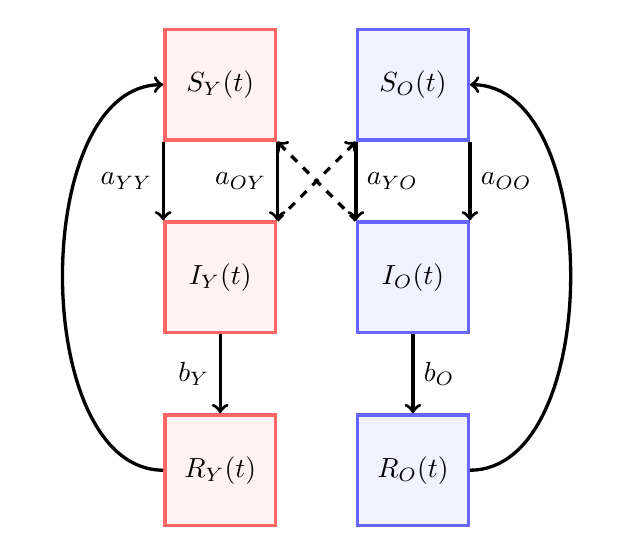
\begin{tikzpicture}[
youngnode/.style={rectangle, draw=red!60, fill=red!5, very thick, minimum size=40},
oldnode/.style={rectangle, draw=blue!60, fill=blue!5, very thick, minimum size=40},
]
%Nodes
\node[oldnode]        (SusO)                            { $S_O(t)$};
\node[oldnode]        (InfO)       [below=of SusO]      { $I_O(t)$};
\node[oldnode]        (RecO)       [below=of InfO]      { $R_O(t)$};

\node[youngnode]      (SusY)        [left=of SusO]      { $S_Y(t)$};
\node[youngnode]      (InfY)        [left=of InfO]      { $I_Y(t)$};
\node[youngnode]      (RecY)        [left=of RecO]      { $R_Y(t)$};

%Lines
\draw[->, very thick] (SusO.south east)  to node[right] {$a_{OO}$} (InfO.north east);
\draw[->, very thick] (InfO.south)  to node[right] {$b_O$} (RecO.north);
\draw[->, very thick] (RecO.east)  .. controls  +(right:17mm) and +(right:17mm)   .. (SusO.east);

\draw[->, very thick] (SusY.south west)  to node[left] {$a_{YY}$} (InfY.north west);
\draw[->, very thick] (InfY.south)  to node[left] {$b_Y$} (RecY.north);
\draw[->, very thick] (RecY.west) .. controls  +(left:17mm) and +(left:17mm)   .. (SusY.west);

\draw[dashed,->, very thick] (InfO.north west)  to  (SusY.south east);
\draw[->, very thick] (SusY.south east)  to node[left] {$a_{OY}$} (InfY.north east);

\draw[->, very thick] (SusO.south west)  to node[right] {$a_{YO}$} (InfO.north west);
\draw[dashed,->, very thick] (InfY.north east)  to  (SusO.south west);
\end{tikzpicture}

\end{document}